\chapter{\dpl\ and \ds\ reconstruction strategy in pp and Pb–Pb collisions}

Due to their mean proper decay lengths (\ct) of 151.2 µm and 309.8 µm respectively~\cite{pdg}, \ds\ and \dpl\ mesons and their charge conjugate cannot be directly detected by the ALICE detector, as they typically decay before reaching the detector. Consequently, their production is inferred through the reconstruction of their hadronic decays into $\ds (\dpl) \rightarrow \mathrm{\phi\pi^+ \rightarrow K^+K^-\pi^+}$ and their charge conjugates, with a branching ratio of $2.21\times10^{-2}$ ($2.69\times10^{-3}$). The spatial resolution capabilities of the ALICE detector~\ref{} allow for the separation of the secondary decay vertices of D mesons from the primary interaction vertex, allowing to conduct an analysis based on the reconstruction and selection of secondary-vertex topologies characterised by relatively large separations from the primary interaction vertex. Furthermore, particle-identification (PID) information are exploited to improve the selection of the D mesons and their decay products and thus to reduce the background.

Two distinct categories of D mesons emerge based on their production mechanisms: \emph{prompt} and \emph{feed-down} D mesons. The former originate directly from the hadronisation of charm quarks or from the strong decay of excited open-charm or charmonium states. Conversely, feed-down D mesons are produced from the decay of hadrons containing a beauty quark. Decay vertices of feed-down D mesons are on average more displaced from the interaction vertex with respect to promptly-produced ones, due to the larger mean proper decay lengths of beauty hadrons (\ct $\sim$ 500 µm~\cite{pdg}) as compared to charm hadrons. Therefore, exploiting the selection of displaced decay-vertex topologies, it is possible not only to separate D mesons from the combinatorial background, but also enables the discrimination between feed-down and prompt D mesons.

\section{Data sample and event selection}
The analyses reported in this Thesis are performed on a dataset of pp collisions at a centre-of-mass energy of \thirteen, collected by the ALICE detector during the 2022 data-taking period and on a dataset of Pb--Pb collision at a centre-of-mass energy per nucleon-nucleon collision of \fivenn collected during 2023. \textcolor{red}{Aggiungere selezioni dei dati e fiducial acceptance!}

\section{\ds and \dpl decay-vertex reconstruction and selection}
\ds\ and \dpl\ mesons (and their charge conjugates) are reconstructed though their hadronic decay channel $\ds, \dpl \rightarrow \mathrm{\phi\pi^+ \rightarrow K^+K^-\pi^+}$. are constructed by combining triplets of tracks with the appropriate charge signs, i.e., (+, --, +) for \ds\ and \dpl\ mesons, and (--, +, --) for their antiparticles. The decay vertex of the candidate is reconstructed through a minimisation of a $\chi^2$-like quantity, denoted as D:
\begin{equation}
    D = \sqrt{\sum_{i=1}^3 \left[\left(\frac{x_i-x_0}{\sigma_{x_i}}\right)^2 + \left(\frac{y_i-y_0}{\sigma_{y_i}}\right)^2 +\left(\frac{z_i-z_0}{\sigma_{z_i}}\right)^2\right]}\quad ,
\end{equation}
where ($x_i,y_i,z_i$) and ($\sigma_{x_i},\sigma_{y_i},\sigma_{z_i}$) represent the position and the uncertainty of the i-th track at the point of closest approach, respectively, while ($x_0,y_0,z_0$) denotes the position of the reconstructed vertex. The invariant mass and momentum of the \ds\ and \dpl\ candidates are computed from the energy and momentum of the measured tracks evaluated at the point of closest approach to the decay vertex. The momentum of the candidate is defined as the sum of the momenta of the three track. For the invariant mass computation, the kaon mass is always assigned to the track with opposite charge sign with respect to the D-meson candidate (\emph{opposite-sign track}). For the two \emph{like-sign tracks}, the two pion-kaon mass hypothesis combinations \big(i.e. ($\mathrm{K^+K^-\pi^+}$) and ($\mathrm{\pi^+K^-K^+}$) for positively charged candidates\big) are considered. 

A lot of triplets can be built from the tracks produced in a pp collision, and this number grows even more in a Pb--Pb collision, where the charged-particles multiplicity is much larger. Thus, many \ds- and \dpl-meson candidates are created, the vast majority of them being combinatorial background. To increase the signal-over-background ratio and the statistical significance of the measurement, tight selections are required. The analyses presented in this Thesis exploit several selection criteria, which can be divided into:
\begin{enumerate}[i]
    \item Track-quality selections
    \item Selections based on the decay topology and kinematics
    \item Particle identification of the decay products
\end{enumerate}

In the following, the applied selections are described in more detalis

\subsection{Track-quality selections}
Only tracks that successfully pass strict quality and kinematic requirements are considered eligible for inclusion in the construction of \ds- and \dpl-meson candidates. In particular, only ITS-TPC tracks with at least 70 (out of \textcolor{red}{XX}) associated space points in the TPC and are selected.\textcolor{red}{Aggiungere info ITS e selezioni di singola traccia}

\subsection{Topological selections}
\ds\ and \dpl\ mesons exhibit a displaced decay vertex topology, which can be used to separate the signal from the uninteresting combinatorial background. Moreover, promptly produced D mesons exhibit different topological features compared to feed-down D mesons, enabling further discrimination between the two production mechanisms. This differentiation potentially offers insights into beauty-quark production through the measurement of open-charm states. These selections are tuned as a function of the \pt\ in order to increase the signal-over-backroung and the statistical significance of the measurement. The different topological selections are presented herein. The corresponding distributions of variables are shown for the signal, which is divided into prompt and feed-down contributions and obtained from Monte Carlo simulations, as well as the combinatorial background, which is obtained in a invariant-mass region away from the signal region, denoted as \emph{sidebands}. \textcolor{red}{Rifare figure cambiando colori e usando le sidebands}

\begin{figure}
    \centering
    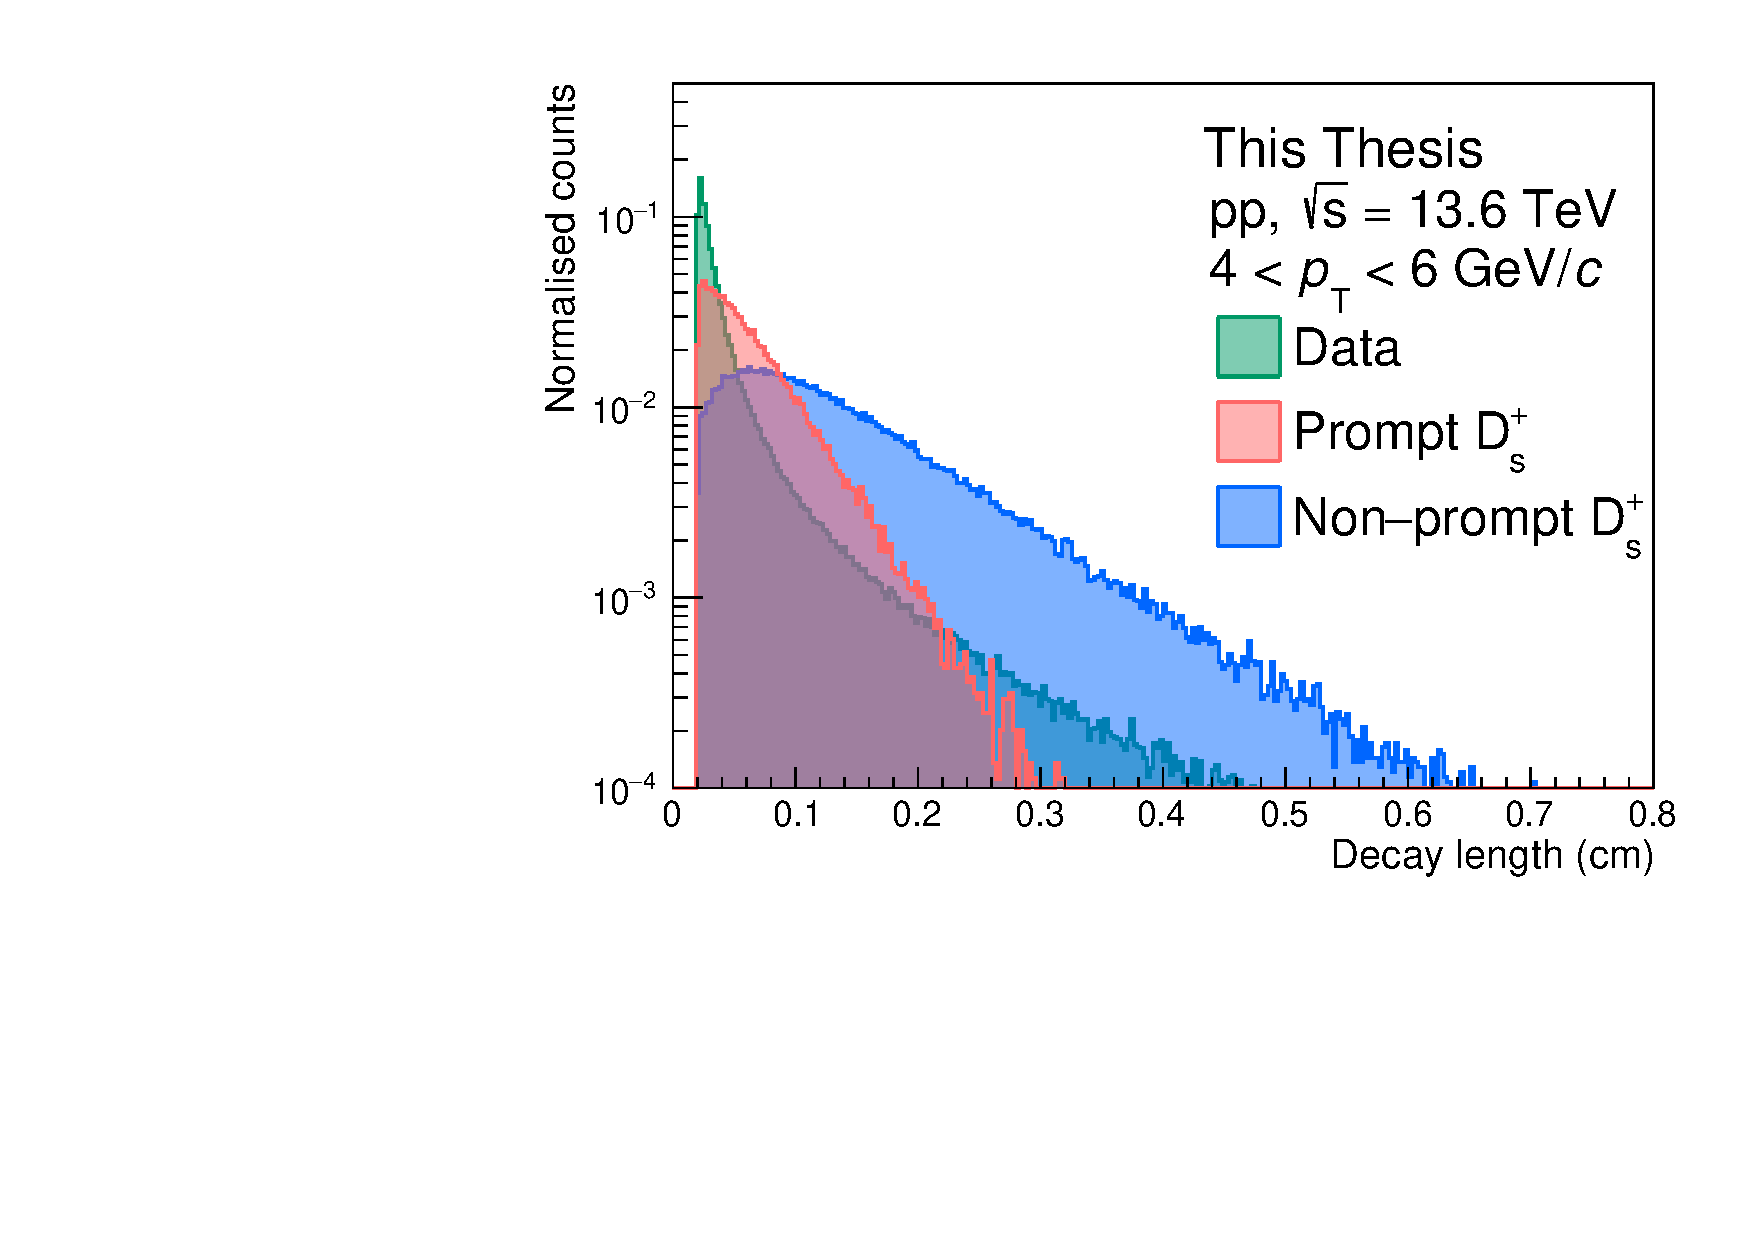
\includegraphics[width=0.48\linewidth]{Figures/Chapter 4/DecayLength.pdf}
    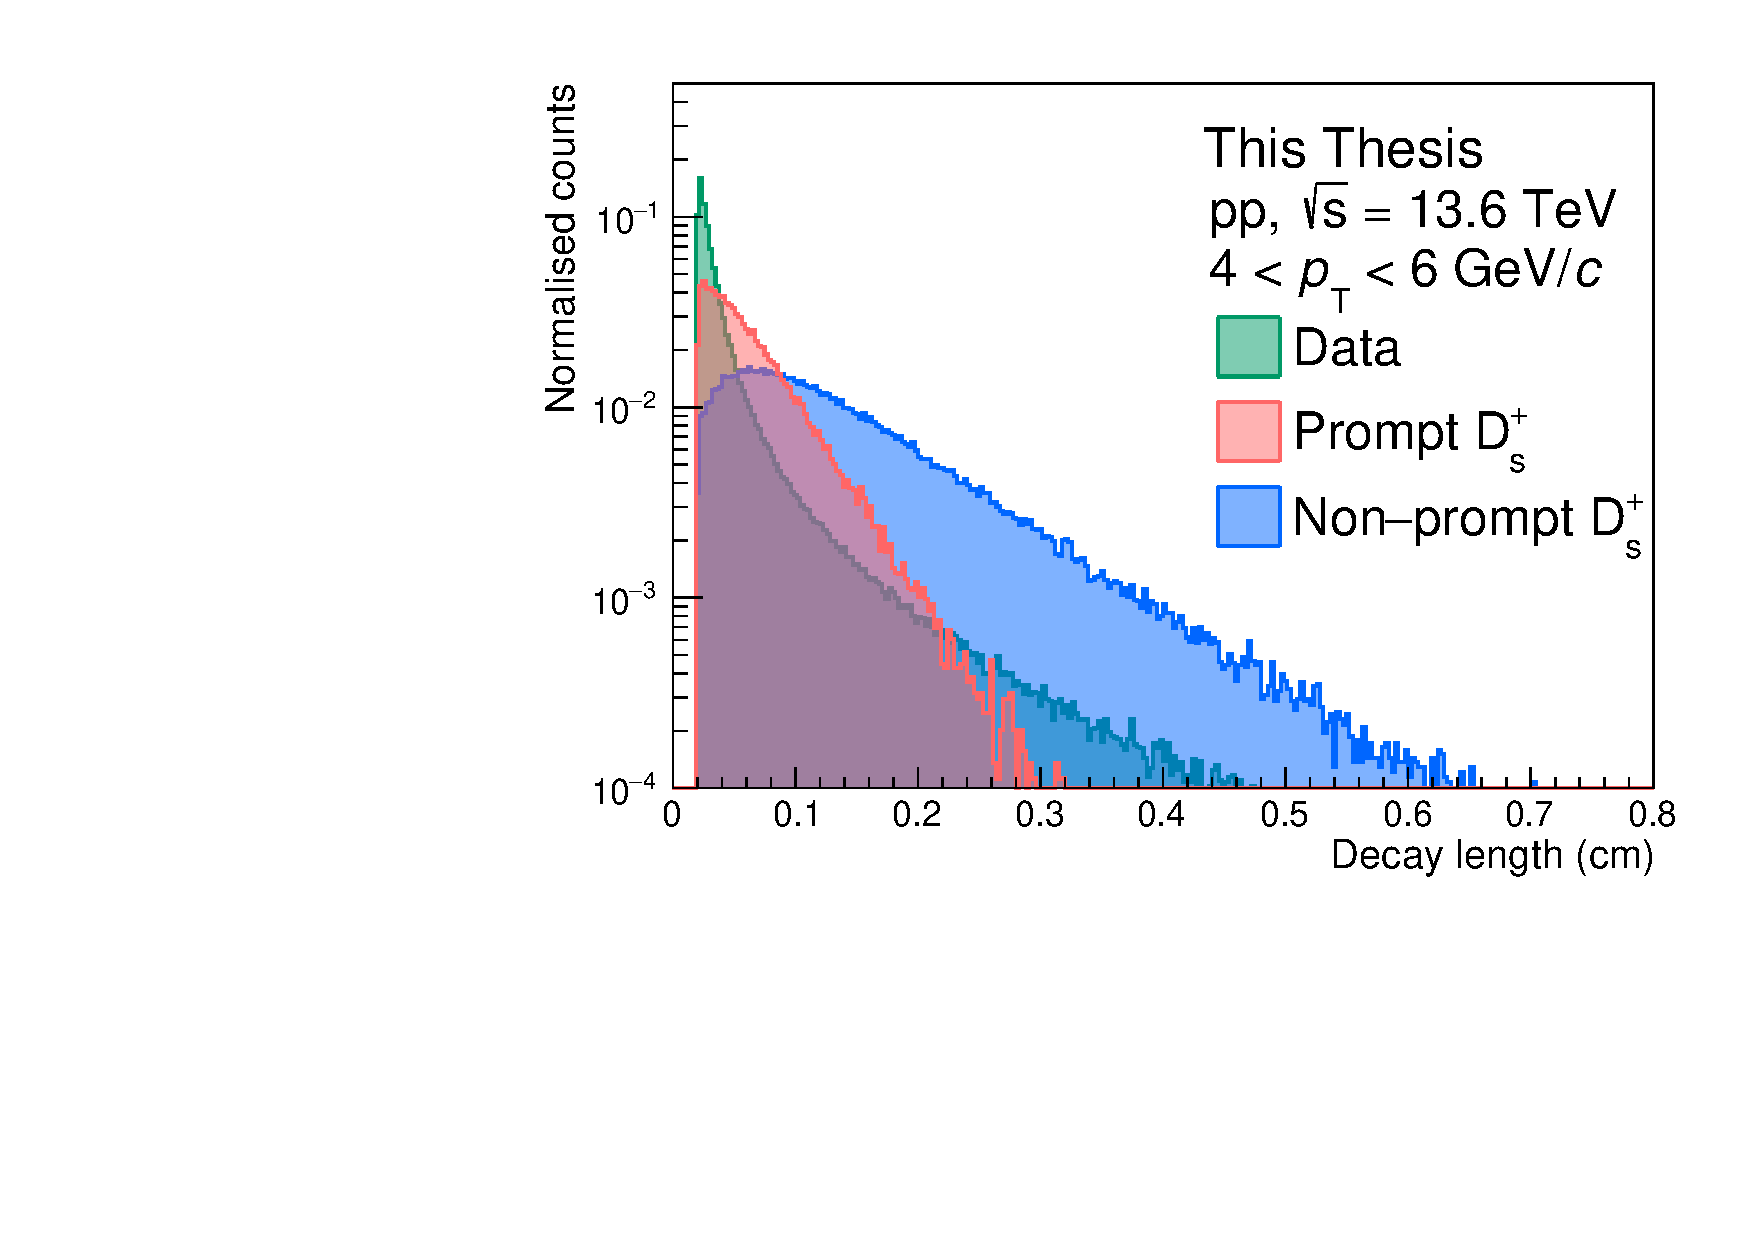
\includegraphics[width=0.48\linewidth]{Figures/Chapter 4/DecayLength.pdf}
    \caption{Caption}
    \label{fig:enter-label}
\end{figure}

\subsubsection{Decay Length}
The decay length is defined as the distance between the primary and secondary vertices. For \ds\ and \dpl\ mesons, the decay length provides an approximation of the actual decay length, as the particle's curvature resulting from the motion in the presence of a magnetic field is not considered. However, given the small mean proper decay length of $\sim 150 (300)$ µm of the \ds\ (\dpl) mesons, this effect is negligible. This is one of the most important variables to distinguish between the signal and the combinatorial background, since the displaced topology of the signal shifts the decay length distribution towards greater values. Furthermore, since beauty hadrons have a larger mean proper decay length than \ds\ and \dpl\ mesons, the feed down decay length distribution is particularly shifted towards lager values, allowing for an easier separation of this production mechanism from the background.  The distribution of the decay length also depends on the \pt\ of the D meson, because of the Lorentz boost which increases the travelled distance in the laboratory reference frame. 
